\documentclass[slovene,11pt,a4paper]{article}

\usepackage[margin=1.5cm,bottom=3cm,foot=1.5cm]{geometry}
\usepackage{amsmath}
\usepackage{booktabs}
\usepackage{float}
\usepackage{graphicx}
\usepackage{changepage}
\usepackage{subcaption}
\usepackage{multirow}
\usepackage{blindtext}
\usepackage{hyperref}
\usepackage[version=4]{mhchem}
\usepackage[slovene]{babel}


\pagenumbering{gobble}

\begin{document}

\title{4. naloga \\ Integracija dinamičnih sistemov v času}
\author{Tadej Lozej 28242023}
\maketitle

\begin{center}
Praktikum strojnega učenja v fiziki \\
\bigskip
Predavatelj: red. prof. dr. Borut Paul Kerševan \\
Asistent: Uroš Perkan
\end{center}

\newpage

\tableofcontents

\newpage

\pagenumbering{arabic}

\section{Uvod}

\section{Lorentzov '63 sistem}

Edward Lorenz je ameriški matematik in meterolog, ki je študiral hidrodinamske sisteme. Je eden začetnikov teorije kaosa. Kaotični sistemi so sistemi katerih rešitev se drastično spremeni pri majhni spremembi začetnih pogojev.

Dinamični sistem, ki ga je študiral Lorenz je poenostavljen opis konvekcije med dvema razsežnima ploskvama z različnima temperaturama. Predpostavimo dvodimenzionalen tok, ki ga opišemo z Navier-Stokesovo enačbo

\begin{equation}
    \frac{\partial \vec{v}}{\partial t} + (\vec{v} \cdot \nabla) \vec{v} = \frac{1}{\rho} \nabla p + \nu \nabla^2 \vec{v} - g \hat{k} \approx -\frac{1}{\rho_0} \nabla p + \nu \nabla^2 \vec{v} + g \beta (T-T_0) \hat{k},
\end{equation}
kjer je $g$ gravitacijski pospešek, $\rho$ gostota zraka, $p$ tlak v tekočini in $\nu = \mu / \rho$ koeficient kinematične viskoznosti.

Prenos toplote pa poteka s konvekcijo in difuzijo

\begin{equation}
    \frac{\partial T}{\partial t} + \vec{v} \cdot \nabla T = \kappa \nabla^2 T,
    \label{eq:KonInDif}
\end{equation}
kjer je $\kappa = \lambda / (\rho c_p)$ konstanta toplotne difuzije. V stacionarnem stanju je temperaturni profil linearen. Med zgornjo hlajeno ploščo pri tempeaturi $T_{cold}$ ter spodnjo ogrevano ploščo $T_{hot}$, ki sta za $H$ narazen bi bil $T_c(z) = T_{hot} - \Gamma z$, kjer je $\Gamma = (T_{hot} - T{cold}) / H$. Enačbo \ref{eq:KonInDif} lahko prepišemo za temperaturne odmike od linearnega profila $\theta (x, y, z) = T(x, y, z) - T_c(z)$ in dobimo

\begin{equation}
    \frac{\partial \theta}{\partial t} - w\Gamma + \vec{v} \cdot \nabla \theta = \kappa \nabla^2 \theta.
    \label{eq:theta}
\end{equation}
S tem prepisom poenostavimo robne pogoje enačbe

\begin{eqnarray}
    \vec{v}(x, y, z) &= 0 \quad \text{za} \quad z = 0, H \\
    \theta (x, y, z) &= 0 \quad \text{za} \quad z = 0, H.
\end{eqnarray}

Če upoštevamo, da je tok nestisljiv ($\nabla \vec{v} = 0$) lahko vektorsko polje hitrosti zapišemo s tokovno funkcijo, tako da velja $\vec{v} = \nabla \times \vec{\psi}$, kjer je $\vec{\psi} = (0, \psi (x, z), 0)^T$. Enačbo \ref{eq:theta} lahko zapišemo s tokovno funkcijo

\begin{equation}
    \frac{\partial \theta}{\partial t} - \frac{\partial \psi}{\partial z} \frac{\partial \theta}{\partial x} + \frac{\partial \psi}{\partial x} \frac{\partial \theta}{\partial z} = \kappa \nabla^2 \theta + \Gamma \frac{\partial \theta}{\partial x}.
\end{equation}
Rešitev lahko poiščemo z 2D Fourierovim razvojem funkcij $\psi$ in $\theta$. V tem primeru dobimo neskončen sistem sklopljenih diferencialnih enačb. Lorentz je reševal takšen sistem a je vzel le minimalno potrebnih koeficientov za nelinearen sistem. V brezdimenzijskih količinah se Lorentzov '63 reduciran sistem enačb glasi

\begin{eqnarray}
    \frac{dX}{d \tau} = \sigma (Y - X) \\
    \frac{dY}{d \tau} = X(r - Z) - Y \\
    \frac{dZ}{d \tau} = XY - bZ,
\end{eqnarray}
kjer je parameter $\sigma = \nu / \kappa$ Prandtlovo število, $r = R/R_c$ je Rayleighovo število in $b = 4 / (1+a^2)$ je pa odvisen od vertikalne razsežnosti plasti. Za vrednosti parametrov $\sigma = 10$, $b = 8/3$ in $r = 28$ je sistem kaotičen.

Rešitve Lorentzovega sistema čez nekaj časa preidejo na nek del prostora, ki mu rečemo atraktor in tam tudi ostane. Rešitev Lorentzovega sistema za naključni začetni pogoj lahko vidimo na sliki \ref{fig:Lorentz}. Pridobljena je bila z numeričnim integratorjem Runge-Kutta četrte stopnje. Rešitev se nepredvidljivo giblje po atraktorju.

\begin{figure}[h!]
    \centering
    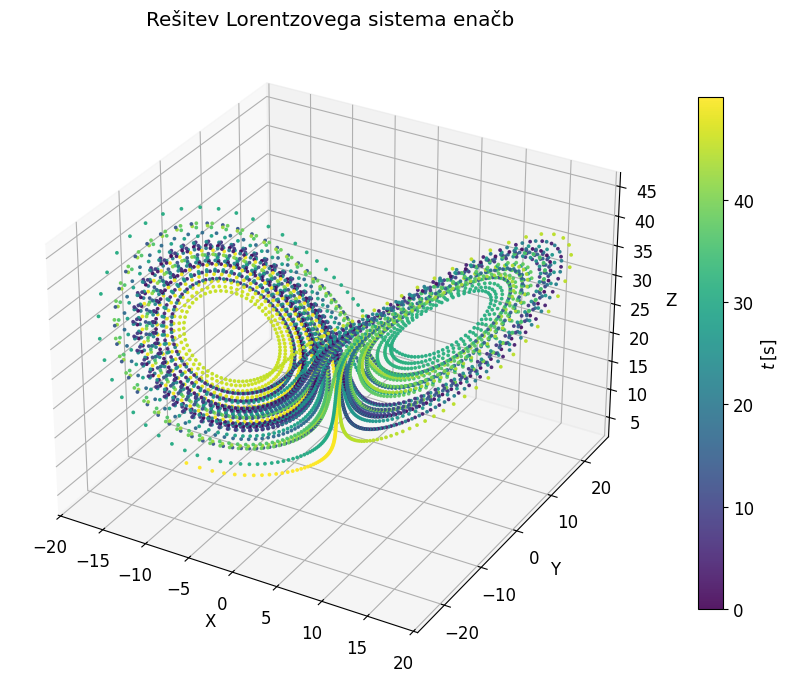
\includegraphics[width = 0.8\linewidth]{imgs/Lorentz.png}
    \caption{Rešitev Lorentzovega sistema.}
    \label{fig:Lorentz}
\end{figure}

Sistem je podobno kot atmosfera nelinearen ter kaotičen. Glavna ideja uporabe nevronskih mrež v meterologiji je pohitritev ter paraleliziranje napovedi.

\subsection{Napovedovanje z RNN mrežo}

Rekurentne nevronske mreže (RNN) se uporabljajo za procesiranje časovnih vrst. Uporabne so predvsem za napovedovanje prihodnosti časovnih vrst, saj so te ponavadi strogo determinirane s prejšnjim stanjem. Lahko si jo predstavljamo podobno kot Kalmanov filter.

Rekurentna nevronska mreža ima v sebi skrito stanje, ki se rekurentno posodablja po vsakem novem prebranem vhodnem vektorju. Skrito stanje deluje kot spomin nevronske mreže, saj vsako novo stanje vsebuje informacijo o preteklih vhodnih podatkih zahvaljujoč skritemu stanju. Rekurentno posodabljanje skritih stanj pa vseeno povzroča hitro izgubo informacij o preteklih vhodih, zato pravimo, da imajo RNN kratkoročni spomin.

Učne podatke pripravimo z integracijo Lorentzovega sistema z numeričnim integratorjem Runge-Kutta četrtega reda. Podatke standardno normaliziramo  ter sekvenciramo. Vhodi v RNN so sekvence dolžine 5, izhodi so pa dolžine 1. Poleg učne množice seveda pripravimo tudi validacijsko množico. 

Pri učenju nevronske mreže uporabimo callbacka \texttt{EarlyStopping} z potrpežljivostjo 10 ter \texttt{RaduceLROnPlateau}. Na sliki \ref{fig:RNN_loss} lahko vidimo učno (modra) ter validacijsko (oranžno) funkcijo izgube pri učenju RNN v logaritemski skali. Pri učenju smo parameter \texttt{batch\_size} postavili na 300. Učna funkcija izgube je kot pričakovano zelo gladka. Presenetilo me je kako malo zašumljena je validacijska funkcija izgube. Mreža se je učila skoraj 250 epochov in funkcija izgube je dosegla vrednost okrog $10^{-6}$. Funkcija izgube je mean squared error (MSE).

\begin{figure}[h!]
    \centering
    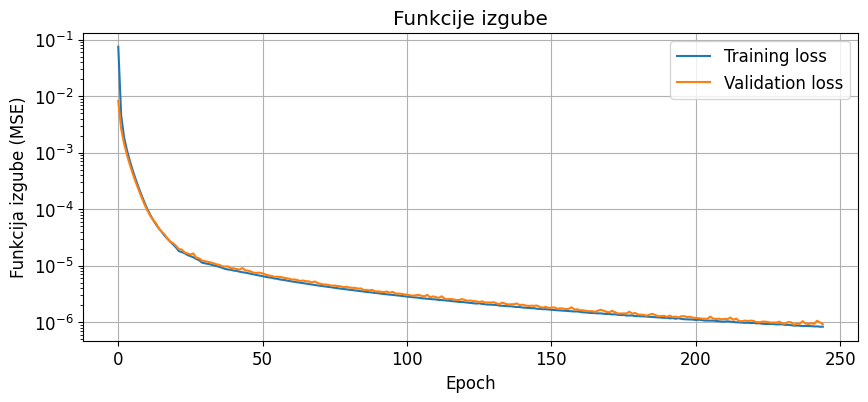
\includegraphics[width = 0.8\linewidth]{imgs/RNN_loss.png}
    \caption{Učna (modra) funkcija izgube ter validacijska (oranžna) funkcija izgube pri učenju RNN.}
    \label{fig:RNN_loss}
\end{figure}

Na sliki \ref{fig:RNN_predict} lahko s polno črto vidimo eno izmed dvesto napovedi v odvisnosti od časa RNN in s črtkano črto rešitve pridobljene z numeričnim integratorjem. Različne barve prikazujejo različne koordinate. Napoved RNN je pridobljena tako, da mu podamo začetno sekvenco nato pa svoje napovedi uporabi za naslednjo napoved. To si lahko predstavljamo kot Kalmanov filter brez izostritve zaradi novih meritev. RNN je seveda v tovrstnih napovedih precej boljša kot Kalmanov filter, a se mi zdi dober za analogijo. Kot pričakovano lahko vidimo, da se napovedi s časom vedno bolj odmikajo od vrednosti dobljene z integratorjem, ki jo bomo vzeli za resnično vrednost. To je smiselno, saj je integrator precej bolj natančna metoda, če sistem diferencialnih enačb poznamo. Prav tako smo mrežo natrenirali na podatkoh dobljenih z integratorjem.

\begin{figure}[h!]
    \centering
    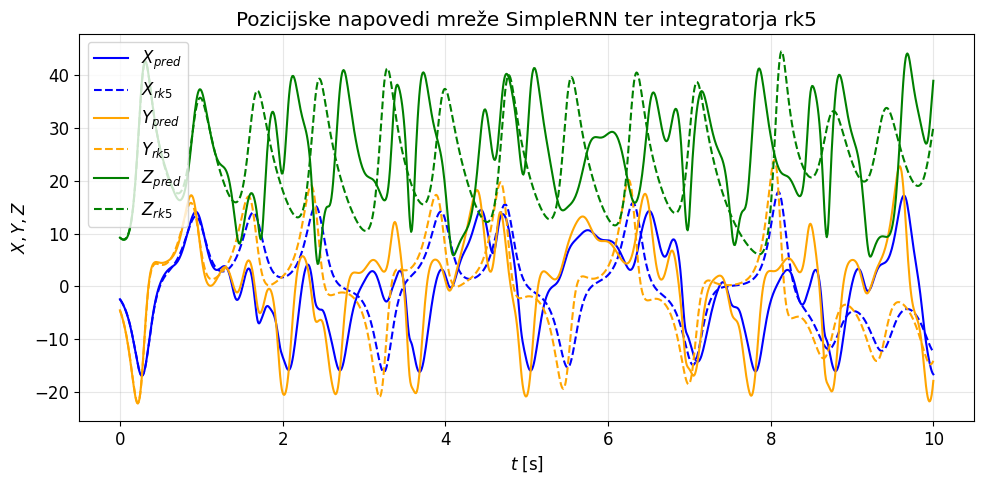
\includegraphics[width = 0.8\linewidth]{imgs/RNN_predict.png}
    \caption{Napovedi Lorentzovega sistema z RNN (polne črte) ter vrednosti pridobljene z integratorjem (črtkane črte). Različne koordinate so prikazane z različnimi barvami.}
    \label{fig:RNN_predict}
\end{figure}

Napako napovedi definiramo kot

\begin{equation}
    E(t) = \sqrt{E_X^2 + E_Y^2 + E_Z^2}; \quad E_\alpha = \sqrt{\frac{1}{N} \sum_{i=1}^{N} (\alpha_{pred} - \alpha_{rk5})^2}
    \label{eq:err}
\end{equation}
kjer je $E_\alpha$ koren iz povprečnege razlike kvadrata med napovedano vrednostjo ter pravo vrednostjo koordinate. Povprečimo čez 200 različnih napovedi. Na sliki \ref{fig:RNN_err} lahko vidimo kako so napake posameznih koordinat ter skupna napaka odvisne od časa. Kot pričakovano vidimo, da s časom napaka narašča. Zanimivo se mi zdi, da se napake v smereh $X$ ter $Y$ ustalijo pri neki vrednosti, napaka v smeri $Z$ pa ne. Mogoče pri več primerih dobimo lezenje v tej smeri.

\begin{figure}[h!]
    \centering
    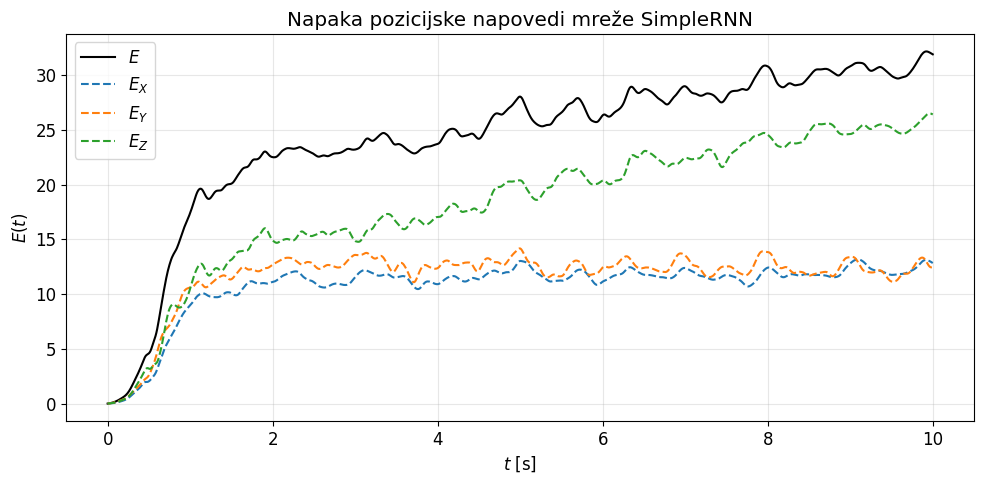
\includegraphics[width = 0.8\linewidth]{imgs/RNN_err.png}
    \caption{Napaka napovedi RN v odvisnosti od časa definirana z enačbo \ref{eq:err}. Z črtkanimi črtami različnih barv so prikazane napake posameznih koordinat.}
    \label{fig:RNN_err}
\end{figure}

\subsection{Napoved z uporabo Luongovega mehanizma pozornosti}

Težavo kratkoročnega spomina lahko rešimo z uporabo Luongovega mehanizma pozornosti. Ta deluje za vse tipe nevronskih mrež, ki so sestavljene iz kodirnika ter dekodirnika. Kodirnik časovno vrsto vhodnih vektorjev preslika v skrita stanja. Običajna RNN bi ta skrita stanja z gosto povezano nevronsko mrežo preslikala v napoved. Glavna ideja Luongovega mehanizma pozornosti se nahaja pri vektorju konteksta. Mreža ta vektor konstruira tako, da primerja tarčno skrito stanje z vsemi skritimi stanji. Vektor konteksta je z utežmi poln vektor. Te uteži določajo linearno kombinacijo kodirnih skritih stanj. Tega nato združimo s tarčnim skritim stanjem in vse skupaj preslikamo v novo skrito stanje, ki je obogateno s kontekstom. To skrito stanje ima osvežen spomin o oddaljenih skritih stanjih.

Učenje mreže z Luongovo pozornostjo poteka na enak način kot učenje RNN. Tudi callbacke ter učne parametre ohranimo enake za boljšo primerjavo modelov, Na sliki \ref{fig:Luong_loss} lahko vidimo učno (modro) ter validacijsko (oranžno) funkcijo izgube. V primerjavi z funkcijami izgube na sliki \ref{fig:RNN_loss} lahko vidimo, da se je model z implementirano Luongovo pozornostjo v manj epochih bolje naučil. Izguba tega modela je v manj kot 200 epochih dosegla vrednost okrog $10^{-7}$. To pomeni, da se je mreža v manj ciklih učenja bolje naučila. To je dober pokazatelj, da je ta model boljši.

\begin{figure}[h!]
    \centering
    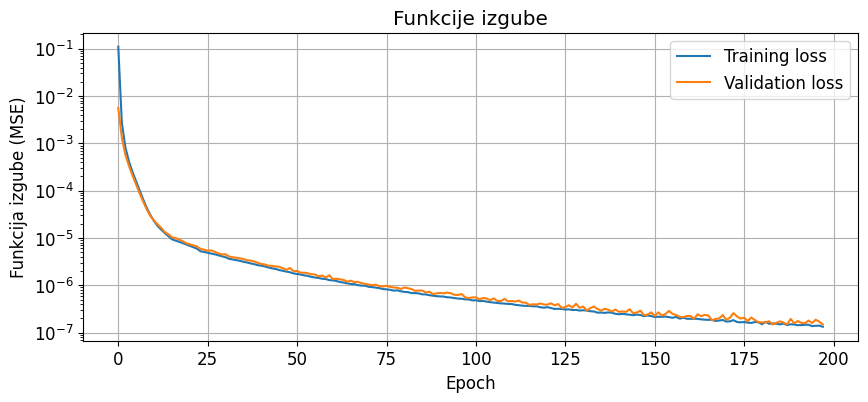
\includegraphics[width = 0.8\linewidth]{imgs/Luong_loss.png}
    \caption{Učna (modra) funkcija izgube ter validacijska (oranžna) funkcija izgube pri učenju mreže z Luongovo pozornostjo.}
    \label{fig:Luong_loss}
\end{figure}

Na sliki \ref{fig:Luong_predict} lahko vidimo primer napovedi iz enakih začetnik pogojev kot pri RNN napovedi na sliki \ref{fig:RNN_predict}. S polno črto vidimo napovedi mreže z Luongovo pozornostjo, s črtkano črto pa realne vrednosti. Z različnimi črtami so prikazane različne koordinate. Vidimo lahko, da je v tem primeru napoved tega modela boljša kot napoved RNN modela. Dlje časa napoved ostane precej natančna.

\begin{figure}[h!]
    \centering
    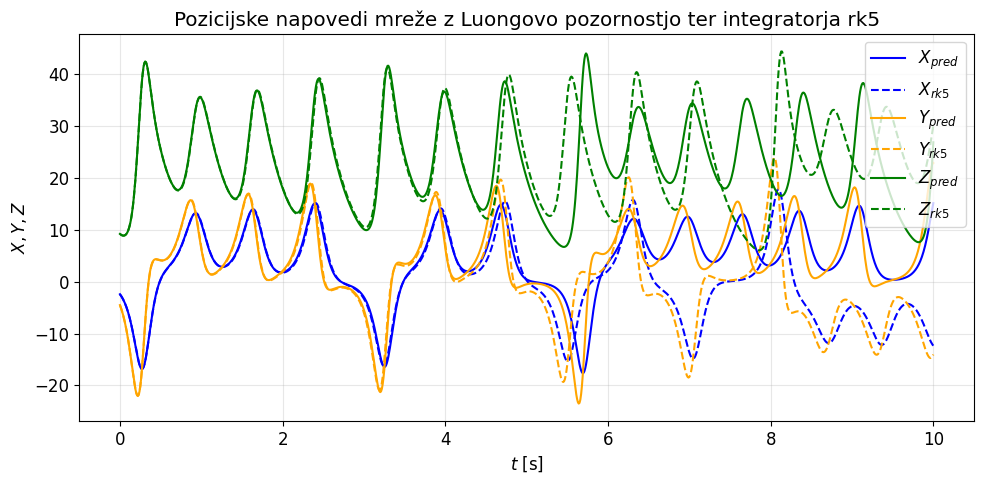
\includegraphics[width = 0.8\linewidth]{imgs/Luong_predict.png}
    \caption{Napovedi Lorentzovega sistema z mrežo z Luongovo pozornostjo (polne črte) ter vrednosti pridobljene z integratorjem (črtkane črte). Različne koordinate so prikazane z različnimi barvami.}
    \label{fig:Luong_predict}
\end{figure}

Napako napovedi mreže z Luongovo pozornostjo v odvisnosti od časa lahko vidimo na sliki \ref{fig:Luong_err}. Napaka je izračunana po enačbi \ref{eq:err}. S črno je prikazana napaka s sivo je pa prikazana napaka v odvisnosti od časa RNN mreže za primerjavo. Lahko vidimo, da je napoved mreže z Luongovo pozornostjo precej natančnejša. S črtkanimi črtami različnih barv lahko vidimo tudi napake posameznih koordinat. Vse koordinate k napaki prispevajo približno enako.

\begin{figure}[h!]
    \centering
    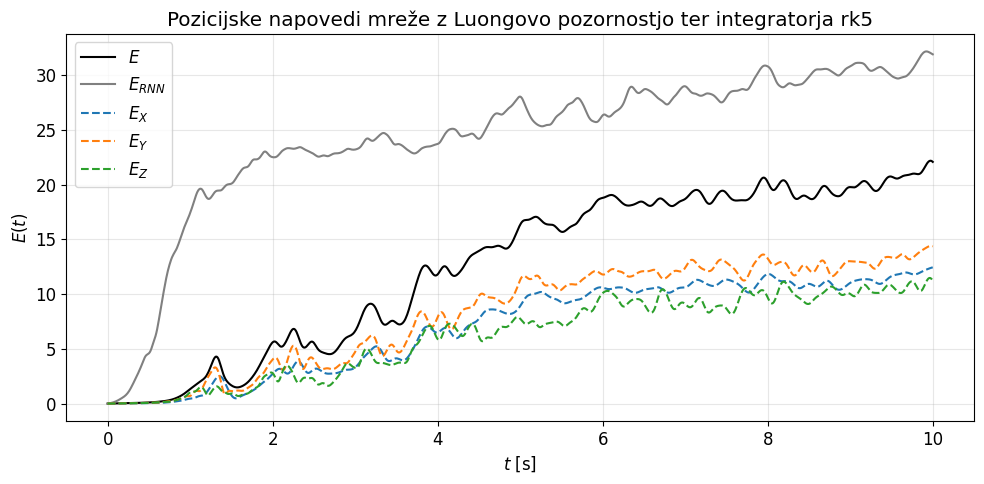
\includegraphics[width = 0.8\linewidth]{imgs/Luong_err.png}
    \caption{Napaka napovedi mreže z Luongovo pozornostjo v odvisnosti od časa definirana z enačbo \ref{eq:err}. Z črtkanimi črtami različnih barv so prikazane napake posameznih koordinat. S sivo barvo je prikazana napaka napovedi RNN mreže za primerjavo.}
    \label{fig:Luong_err}
\end{figure}

\subsection{Iskanje optimalnih hiperparametrov}

\end{document}